% Double-blind 8-page version for FCCM (Part I only), made from odin3.tex by a script: authors,
% self-citations (blind.bib), repository URLs, the tool and suite names (placeholders AnonSynth, AnonSuite, ...) withheld;
% figures from IMAGE/blind/. On acceptance use odin3.tex.
% Companion file: odin3.tex is the same paper with authors and names restored; this blind
% copy is the version submitted to the conference, and the non-blind copy is used on acceptance.
% AnonSynth paper draft. IEEEtran conference class; compiles with pdfLaTeX (Overleaf) and BibTeX.
% Companion files: anonsynth_blind.tex is this same paper anonymized for double-blind review and is
% the version submitted to the conference; this non-blind copy is used if the paper is accepted.
% Figures are TikZ (IMAGE/fig_*.tex, sharing IMAGE/odin3-tikz-styles.tex) except fig_ast, a
% hand-drawn SVG converted to IMAGE/fig_ast.pdf (see README.md). Every number below is taken
% from the repository's docs (DESIGN.md, IR.md, PHASE0-7.md, specs/, RELEASE-NOTES-1.0.md, CHANGELOG.md, and ADR D10 and D11 for the v1.0 scope) and git log as of
% v1.0.0 (tagged 2026-10-21; the cost is as of the v1.0 close); the release status is v1.2.0 (2026-10-28, CHANGELOG.md, docs/V1.1.1.md, docs/V1.2.0.md). The M2 QoR ratios come from the vtr-qor table
% 20261020-1642-M2 (published to anonsynth-golden, qor/3c9a4d23b27d/M2), the cost from
% docs/log_cost_of_tokens_and_time-v1.0.md (the frozen v1.0 count).
% Structure (step 2 rewrite, 2026-10-28): Part I = Introduction, Background (with the Glossary, glossary.tex),
% The Innovations, Methodology, Experiments (one subsection per hypothesis), Discussion, Future Work, Conclusion,
% then the references; Part II (after the references) is the system in detail; Appendix A is the research log
% (register.tex, every hypothesis one row). glossary.tex and register.tex are generated (make_glossary.py, make_register.py).
\documentclass[conference]{IEEEtran}

\usepackage{cite}
% A key cited in both lists gets the same number in both, so a repeated \bibcite is not an error.
\makeatletter\def\bibcite#1#2{\global\@namedef{b@#1}{#2}}\makeatother
\usepackage{amsmath}
\usepackage{graphicx}
\usepackage{booktabs}
\usepackage{array}
\usepackage{url}
\usepackage{listings}
\usepackage{tikz}
\usetikzlibrary{positioning,fit,arrows.meta,shapes.geometric,backgrounds,calc,matrix}

\graphicspath{{IMAGE/}}
% Shared figure palette and styles; each figure is IMAGE/fig_<name>.tex, pulled in with \input.
% Shared TikZ styles for the Odin III paper figures (IMAGE/fig_*.tex).
% Needs: \usepackage{tikz} and
%   \usetikzlibrary{positioning,fit,arrows.meta,shapes.geometric,backgrounds,calc,matrix}
% loaded first (odin3.tex and IMAGE/figures.tex both do). Input this file once, in the preamble.
%
% Palette: the greens and browns of a tree and its greenery, with black for Odin's raven as the
% strong ink. Green = ColorBrewer "Greens", brown = a warm earth ramp. Text is dark on the light
% fills and white only on the dark browns and the black. Build status is coded twice, by fill and
% by border, so it survives a black-and-white print:
%   built        mid-green fill,  solid dark-green border
%   in progress  pale-green fill, solid green border
%   specified    white fill,      dashed green border
%   planned      white fill,      dotted brown border

% ---- colours ------------------------------------------------------------------------------
\definecolor{o3ink}{HTML}{111111}      % text and arrows: the raven's black
\definecolor{o3sub}{HTML}{4E342E}      % secondary text (sub-project tags, notes): dark brown
\definecolor{o3grn9}{HTML}{00441B}
\definecolor{o3grn8}{HTML}{006D2C}
\definecolor{o3grn7}{HTML}{238B45}
\definecolor{o3grn5}{HTML}{74C476}
\definecolor{o3grn4}{HTML}{A1D99B}
\definecolor{o3grn3}{HTML}{C7E9C0}
\definecolor{o3grn2}{HTML}{E5F5E0}
\definecolor{o3grn1}{HTML}{F7FCF5}
\definecolor{o3brn9}{HTML}{3E2723}     % root system, dark brown (white text only)
\definecolor{o3brn8}{HTML}{5D4037}
\definecolor{o3brn7}{HTML}{4E342E}
\definecolor{o3brn6}{HTML}{6D4C41}     % trunk
\definecolor{o3brn5}{HTML}{8D6E63}
\definecolor{o3brn4}{HTML}{C9B6A4}     % branches, lighter brown
\definecolor{o3brn3}{HTML}{E0D3C6}
\definecolor{o3brn2}{HTML}{F1E9DF}
\definecolor{o3brn1}{HTML}{F8F4EE}

% ---- text helpers -------------------------------------------------------------------------
% A second, smaller line in a node: \odinsub{2C}.
\newcommand{\odinsub}[1]{{\scriptsize\color{o3sub}#1}}
% Code names inside figures (the paper's \code is not defined in the standalone build).
\newcommand{\odintt}[1]{\texttt{#1}}

% Scale a figure down only if it is wider than #1 (it never scales up). Each figure is drawn
% at its print size, so this is a safety net; a scaled figure writes "ODINFIT" to the log.
\newsavebox{\odinfigbox}
\newcommand{\odinfit}[2]{%
  \sbox{\odinfigbox}{\ignorespaces#2\unskip}%
  \ifdim\wd\odinfigbox>#1\relax
    \typeout{ODINFIT: figure scaled from \the\wd\odinfigbox\space to \the#1}%
    \resizebox{#1}{!}{\usebox{\odinfigbox}}%
  \else
    \usebox{\odinfigbox}%
  \fi}

% ---- TikZ styles --------------------------------------------------------------------------
\tikzset{
  % every figure
  odin/.style={font=\footnotesize, color=o3ink, line join=round,
               >={Stealth[length=3.4pt, width=2.8pt]},
               % node text breaks the same way in any class: no hyphens, loose lines rather than overfull
               execute at begin node={\hyphenpenalty=10000\exhyphenpenalty=10000%
                 \tolerance=9999\emergencystretch=10pt}},
  % shapes
  box/.style={draw, rectangle, rounded corners=1.6pt, align=center, line width=0.55pt,
              inner xsep=2.5pt, inner ysep=2pt, minimum height=6.5mm},
  store/.style={draw, cylinder, shape border rotate=90, aspect=0.16, align=center,
                line width=0.55pt, inner xsep=2pt, inner ysep=1pt, minimum height=8mm},
  plain/.style={align=center, inner sep=1pt},
  % build status (combine with a shape: [box, built])
  built/.style={fill=o3grn4, draw=o3grn8, solid},
  inprog/.style={fill=o3grn2, draw=o3grn7, solid},
  spec/.style={fill=white, draw=o3grn7, dash pattern=on 2.4pt off 1.4pt},
  planned/.style={fill=white, draw=o3brn5, dash pattern=on 0.6pt off 1.3pt,
                  line width=0.75pt},
  % neutral fills for structure figures
  neutral/.style={fill=o3brn2, draw=o3brn6, solid},
  light/.style={fill=o3grn1, draw=o3grn7, solid},
  external/.style={fill=o3brn2, draw=o3brn6, dash pattern=on 3pt off 1.2pt on 0.6pt off 1.2pt},
  emph/.style={line width=1.3pt},
  % grouped regions, drawn on the background layer
  region/.style={draw=o3brn4, fill=o3brn1, rounded corners=3pt, line width=0.5pt,
                 inner sep=4pt},
  bluregion/.style={draw=o3grn3, fill=o3grn1, rounded corners=3pt, line width=0.5pt,
                    inner sep=4pt},
  regionlabel/.style={font=\scriptsize\bfseries, color=o3brn7, inner sep=1.5pt},
  % arrows
  flow/.style={->, line width=0.55pt, draw=o3ink},
  flowplanned/.style={->, line width=0.6pt, draw=o3brn6, dash pattern=on 0.6pt off 1.3pt},
  ref/.style={->, line width=0.5pt, draw=o3grn8, dash pattern=on 2.4pt off 1.4pt},
  edgelabel/.style={font=\scriptsize, color=o3sub, inner sep=1pt, fill=white},
  % records: a header row and field rows, built with \matrix (see fig_ir_model.tex)
  record/.style={matrix of nodes, ampersand replacement=\&, row sep=-\pgflinewidth,
                 inner sep=0pt, nodes={draw=o3brn6, line width=0.5pt, fill=white,
                 font=\scriptsize, anchor=center, align=left, inner xsep=2.5pt,
                 inner ysep=1.2pt, minimum height=4.4mm}},
  rechead/.style={fill=o3grn3, font=\scriptsize\bfseries, align=center},
  % legend keys
  legendkey/.style={box, minimum width=4.2mm, minimum height=2.6mm, inner sep=0pt},
  legendtext/.style={font=\scriptsize, inner sep=1pt, text height=1.5ex, text depth=0.3ex},
}

% \odinlegend{<node options, e.g. anchor=north east, at={(x,y)}>}
% The build-status key, one row, as a single node so figures can place it like any node.
\newcommand{\odinlegend}[1]{%
  \matrix[ampersand replacement=\&, column sep=1.2pt, inner sep=2pt, draw=o3brn4,
          rounded corners=2pt, fill=white, line width=0.4pt, #1]{%
    \node[legendkey, built]{};   \& \node[legendtext]{built};       \& \node{\hspace{3pt}}; \&
    \node[legendkey, inprog]{};  \& \node[legendtext]{in progress}; \& \node{\hspace{3pt}}; \&
    \node[legendkey, spec]{};    \& \node[legendtext]{specified};   \& \node{\hspace{3pt}}; \&
    \node[legendkey, planned]{}; \& \node[legendtext]{planned};     \\
  };}

% \odinrecord{<name>}{<matrix options: position, nodes={text width=...}>}{<header>}{<rows>}
% A record (struct) as a one-column matrix: a header cell, then one cell per field, rows
% separated by \\ and ended by \\. Cells are <name>-<row>-1, so edges can leave from a field.
\newcommand{\odinrecord}[4]{%
  \matrix[record, #2] (#1) {|[rechead]| #3 \\ #4};}


% A visible marker for gaps: numbers not yet measured, text Peter must supply.
\newcommand{\todo}[1]{\textbf{[TODO: #1]}}
% Names from the code base.
\newcommand{\code}[1]{\texttt{#1}}

\lstset{basicstyle=\ttfamily\scriptsize, columns=fullflexible, keepspaces=true,
        frame=single, framesep=2pt, xleftmargin=3pt, xrightmargin=3pt,
        aboveskip=4pt, belowskip=4pt}

\begin{document}


% Earlier title: "AnonSynth: A Provenance-Tracked HDL Elaboration and Front-End Synthesis Framework
% for FPGA CAD Research".
\title{AnonSynth, the Final Frontier:\\
Verilog Synthesis for FPGAs\\Built by the DarkFactory and Leads to AnonSuite}

\author{\IEEEauthorblockN{Anonymous Author(s)}
\IEEEauthorblockA{Affiliation withheld for double-blind review}}

\maketitle

\begin{abstract}
Odin was written in 2005 and Odin~II in 2010. Odin~II became the Verilog front end of the VTR FPGA CAD flow, and Yosys with the Parmys plugin has since displaced it. After the ``MAIking software'' moment of December 2025, when AI coding agents began to make real software, I asked the final-frontier question: could a Dark Factory, in which agents turn a human's specification into software, build AnonSynth, matching Odin~II's good ideas and plugging into the VTR flow? AnonSynth (MIT license) is a C17 framework with one provenance-tracked IR, two-stage elaboration, re-implementations of Yosys~0.55's \code{proc}, \code{opt}, \code{fsm}, \code{wreduce} and \code{flatten}, architecture-driven partial mapping, linked ABC and VPR-ready BLIF, a SystemVerilog front end over the slang library, and a versioned C ABI for plugins and AI tools. Each claim of the paper is a hypothesis with an experiment that confirms it or not. Confirmed: every netlist AnonSynth produced for the 15 VTR benchmarks that fit the development laptop routes in VPR, with geomean CLB, channel-width, delay and wirelength ratios against the Parmys flow inside a 1.20 gate; refinement proofs, functional checks and byte-identical reruns hold; checking against oracles found defects in the Parmys flow; and v1.2.0 records the chain of HDL constructs behind every object. Not confirmed: recording constructs at elaboration costs more than 5\% of read time on two of five large designs, so it is off by default; equivalence on the 14 small VTR designs is only partly proved. Power is not measured. I state the caveats of this MAIking: a human watched every day, the code has not been deeply read by a human, and testing covers a subset of scenarios. I report the time and token cost, and present the AnonSuite ecosystem that this approach made possible.
\end{abstract}

\begin{IEEEkeywords}
FPGA CAD, HDL elaboration, Provenance, VTR, AI coding agents, DarkFactory
\end{IEEEkeywords}

% ==========================================================================================
% PART I: the FCCM paper (about 8 pages plus references)
% ==========================================================================================

% ------------------------------------------------------------------------------------------
\section{Introduction}
\label{sec:intro}

% Plain-English problem. Each term is defined where it is first used (tag def:<key>), in the order
% of glossary.tex (make_glossary.py); Sec. Background repeats them with the source of the definition.
\emph{The problem in plain English.}
An FPGA is a chip of programmable logic blocks and wires onto which a digital design is loaded. % def:fpga
Its storage cell is the flip-flop, which keeps one bit between clock edges, % def:ff
and its logic cell is the LUT (look-up table), a small memory that computes any function of six inputs and, with a flip-flop, forms the basic logic element. % def:lut
LUTs and flip-flops are grouped into CLBs (configurable logic blocks), which are placed as one unit~\cite{luuthesis}. % def:clb
A designer describes the circuit in a hardware description language (HDL), here Verilog, % def:hdl
and a tool turns that text into a netlist, the list of gates, LUTs and other cells and the wires between them. % def:netlist
The tool that does the first part of this job is the synthesis front end. % def:front
Its first step, elaboration, resolves parameters, generate loops and hierarchy and turns the parsed HDL into a design graph. % def:elab
ABC then maps the gates of the netlist onto LUTs~\cite{brayton2010abc}. % def:abc
After that, packing groups the LUTs and flip-flops into CLBs, placement chooses a site on the chip for each CLB, and routing chooses the wires between them. % def:prp
The open-source flow that does all of this is VTR (Verilog-to-Routing), and VPR is its packing, placement and routing program~\cite{rose2012vtr,luuthesis}. % def:vtr
A front end that gives VTR good results is not enough for the research I want to do. % why
Synthesis changes the designer's structure: it flattens hierarchy, merges and splits operators, and covers logic with LUTs that no source line names. % why2
The link from each object of the final netlist back to the HDL that produced it is its provenance, % def:prov
and no front end that serves VTR keeps it.

\emph{Why AnonSynth.}
Odin~\cite{jamieson2005odin} started from nothing. It used Icarus Verilog~\cite{icarus} as the front end, but Icarus treats Verilog as a simulation language, and building synthesis on a simulator's front end cost a year of work to learn the basics of Verilog synthesis. Odin~II~\cite{jamieson2011odin2} followed and wrote a proper compiler front end: a Bison and Flex parser, and elaboration into a flattened netlist. Odin~II became the Verilog front end of the VTR flow~\cite{rose2012vtr,luu2014vtr7}, and it mapped multipliers, memories, and adders onto the dedicated blocks that an architecture file describes. VTR has since moved its default front end to Parmys~\cite{parmys}, an extension of Yosys~\cite{wolf2013yosys,yosys} that carries Odin~II's mapping of multipliers, memories and adders onto dedicated blocks, and the VTR documentation now marks Odin~II as deprecated. % def:odin2

Then came what I call the ``MAIking software'' moment of December 2025: AI coding agents~\cite{claudecode} became able to make real software. Yu and Ren's multi-agent self-evolved ABC~\cite{yu2026selfevolvedabc} showed that LLM agents can change the source of a million-line logic synthesis system, rebuild it, check it, and keep the changes that improve its results; VPR-Evolve~\cite{wu2026vprevolve} has since done the same for FPGA place and route, and Ding et al.\ survey high-level synthesis in the agentic era~\cite{ding2026hlsagentic}. Those works build on existing tools, and together they raised the final-frontier question I had to ask. Dan Shapiro describes five levels of AI-assisted programming; at the last, the Dark Factory, the software process is ``a black box that turns specs into software''~\cite{shapiro2026darkfactory}. % def:dark
Could I use a Dark Factory to build AnonSynth, a front end that matches Odin~II's good ideas and plugs into the VTR flow where Yosys has displaced Odin~II? This paper describes the answer to that question (YES!), what has been built to answer it, and how it is tested. AnonSynth is public (URL withheld for review).

\emph{What counts as a good result.}
A front end is judged on several measures at once, and the dataset I want from it must carry all of them.
The routing channel width is the number of wire tracks per channel that the router needs, written $W$; % def:minw
the wirelength is the total length of wire the routed design uses; % def:wl
the critical path is the slowest path between registers, and its delay is the critical-path delay (CPD); % def:cpd
a near-critical path is one whose delay is within a stated window of the CPD. % def:near
Area is how much chip a design uses: its LUTs, its CLBs and $W$, and a good result keeps it low. % def:area
Speed is how fast the circuit runs: the CPD and the wirelength, and where available the near-critical paths, and a good result keeps it high, on the critical and on the near-critical paths alike. % def:speed
Power is the energy the circuit uses, and a good result keeps it low; this paper does not measure power. % def:power
The reason for the provenance link is the AnonData dataset (Fig.~\ref{fig:yggdrasil}): a record that shows \emph{why} each structure was placed where it was, through the HDL construct it came from, for all of these measures at once.

\emph{Claims and experiments.}
Each claim in this paper is a hypothesis, a statement that an experiment can confirm or fail to confirm. % def:hyp
The experiment gives a verdict: USEFUL (confirmed under the stated gate or check), POSSIBLY GOOD (confirmed but narrow or fragile, so stated with the fragility and never as proof alone), INCONCLUSIVE (neither confirmed nor failed), or DISMISSED (failed). Sec.~\ref{sec:results} gives each confirmed hypothesis its experiment. A failed one is reported in the Discussion.

\emph{The innovations in plain English.}
\begin{enumerate}
\item \textbf{A front end that plugs into VTR.} A program that reads Verilog and hands a netlist to VTR, so ABC, packing, placement and routing work as before and the result is about as good as with the Yosys-based front end, comparable and not equal.
\item \textbf{Checking against oracles.} Every stage is compared with a trusted reference tool, an oracle, % def:oracle
and where the two disagree a probe decides which one matches the Verilog, so the reference's own mistakes surface.
\item \textbf{One provenance-tracked IR.} Every object remembers which Verilog text made it, through every pass, in one internal design graph, the IR (intermediate representation), % def:ir
and from v1.2.0 it remembers the whole chain of constructs, including the places where two constructs were blended.
\item \textbf{A versioned C ABI.} A stable interface (the ABI) so a plugin, a separately built program that adds features, and AI tools can drive and read AnonSynth without changing it. % def:abi
\end{enumerate}
The way AnonSynth was built, with a Dark Factory, is the method and context of the paper and not a tested innovation (Sec.~\ref{sec:method-built}).

\emph{Contributions.} The contributions are the innovations with the hypotheses that confirmed them:
\begin{itemize}
\item the front end and its flow: all 15 designs that fit the laptop route, with average ratios inside a stated bound against Parmys (O1, USEFUL), on a baseline that reproduces VTR's own results (O2, USEFUL; Sec.~\ref{sec:q-qor});
\item checking against oracles: a proof that the lowering pass keeps the design's behaviour, with no unexpected result (O4, USEFUL), a functional check that passes on 12 of 15 designs (O6, USEFUL), identical output on rerun (O7, USEFUL), 144 of 156 VerilogEval references run through the gate flow (O8, USEFUL), and six defects found in the Parmys flow (O9, USEFUL; Secs.~\ref{sec:q-proof} to \ref{sec:parmys-bugs});
\item provenance: the chain of constructs recorded at every granularity and read back (O14, USEFUL), and a timing attribution that does not change VPR's result (O17, POSSIBLY GOOD, on three designs); the cost of recording constructs at elaboration failed its gate (O16, DISMISSED), and the round trip of exports is only partly shown (O15, INCONCLUSIVE; Secs.~\ref{sec:q-prov} to \ref{sec:q-timing});
\item an account of the build with a Dark Factory under daily human oversight, with its time and token cost and its limits (Sec.~\ref{sec:method-built});
\item a presentation of AnonSuite, the suite this approach made possible, including a reimplementation of an earlier Verilog teaching game~\cite{anon01}, now called AnonGame.
\end{itemize}

The approach has limits, and I state them first. It was not a lights-out factory. I watched the agents build and interacted with them daily: I wrote the design specification and goals, ruled on every design rule (architecture decisions, IR invariants, mapping algorithms), and managed the risks of a small machine. Everything ran on one Windows desktop (Intel i7-13700) inside a WSL2 virtual machine with 12 logical processors and 23\, GiB of memory, where an out-of-memory condition or a full host disk kills the virtual machine and every agent in it. Heavy jobs therefore run one at a time under a machine-wide lock in a memory-capped slice, and the largest VTR designs were shipped out to a bigger machine instead of being run. The codebase has not been deeply read by a human. It took 14 calendar days to reach version~1.0 (first commit 2026-10-08, v1.0.0 released 2026-10-21, both days counted) and was tested with a subset of the possible scenarios. Odin~II and Yosys with Parmys are production oracles, so more testing is always possible. We found defects in the Parmys flow (Sec.~\ref{sec:parmys-bugs}), which we will report to those projects in good faith, because we want to contribute to these open-source CAD tools.

The community may object to such a process. It may also ask a harder question: if a guided Dark Factory with oracles can rebuild a tool like this, could a reverse-engineering process let open-source tools rip out the human-years of engineering behind today's EDA tool landscape? (To the companies, I would suggest moving to a cloud service model as soon as possible.) My goal is narrower: to run experiments I couldn't do with Yosys, and with AnonSynth I can now, and the ideas I hoped my students could pursue were limited by inflexibilities in the toolflow.

I call this new suite AnonSuite (Fig.~\ref{fig:yggdrasil}). AnonSynth is the trunk: its steps run from the roots (Verilog and netlists in) to the crown (a netlist for VTR out), and every path passes through its one provenance IR, which is why I see it as a final frontier. The oracles (Yosys, Parmys, Odin~II, VTR's stored results, and ABC) stand as a small forest beside the trunk, to compare against. Three deep roots reach three wells of outside work: prior work, FPGA CAD and its views, and synthesis sources. In the canopy are AnonGUI (the experiment runner and GUI); AnonSim (the simulation bridge); and AnonGame, a port of an earlier Verilog teaching game~\cite{anon02}, which AnonGUI connects to. AnonData, the circuit knowledge base, hangs there as the fruit: the dataset harvested from the runs, which answers why things are where they are, through provenance. Side branches carry tools and experiments: AnonRE (reverse engineering) continues earlier netlist-to-RTL work~\cite{anon03} with an LLM-free L0-L2 flow (provenance datasets, a Bayesian signal-role classifier, clustering and graph-network reconstruction), now measured against the baseline's own metrics; AnonHT (hardware Trojan detection tools); AnonPlace, an earlier placement experiment~\cite{anon04,anon05}, redone with provenance (Sec.~\ref{sec:provenance-problem}); and AnonTrace~III (the Micro through the Macro), a record-and-replay walk of an AnonSynth run. All the code is public (URL withheld for review).

\begin{figure*}[tp]
\centering
\scalebox{0.66}{\odinfit{\textwidth}{% AnonSuite drawn as a tree. Roots (dark brown) at the bottom: what AnonSynth reads and writes, and the
% tools it links to. The trunk (brown) is AnonSynth, its steps running DOWN from parse to the roots. A small
% forest of mini trees on the right holds the oracles, to compare against. The canopy (green oval) is the
% tree-top: AnonGUI, AnonSim (the arrow to AnonGame) and AnonGame (verilogTown). AnonRE,
% AnonHT, AnonPlace and AnonTrace III are side branches off the trunk, tools and experiments.
% No status; the GitHub links are in the caption.
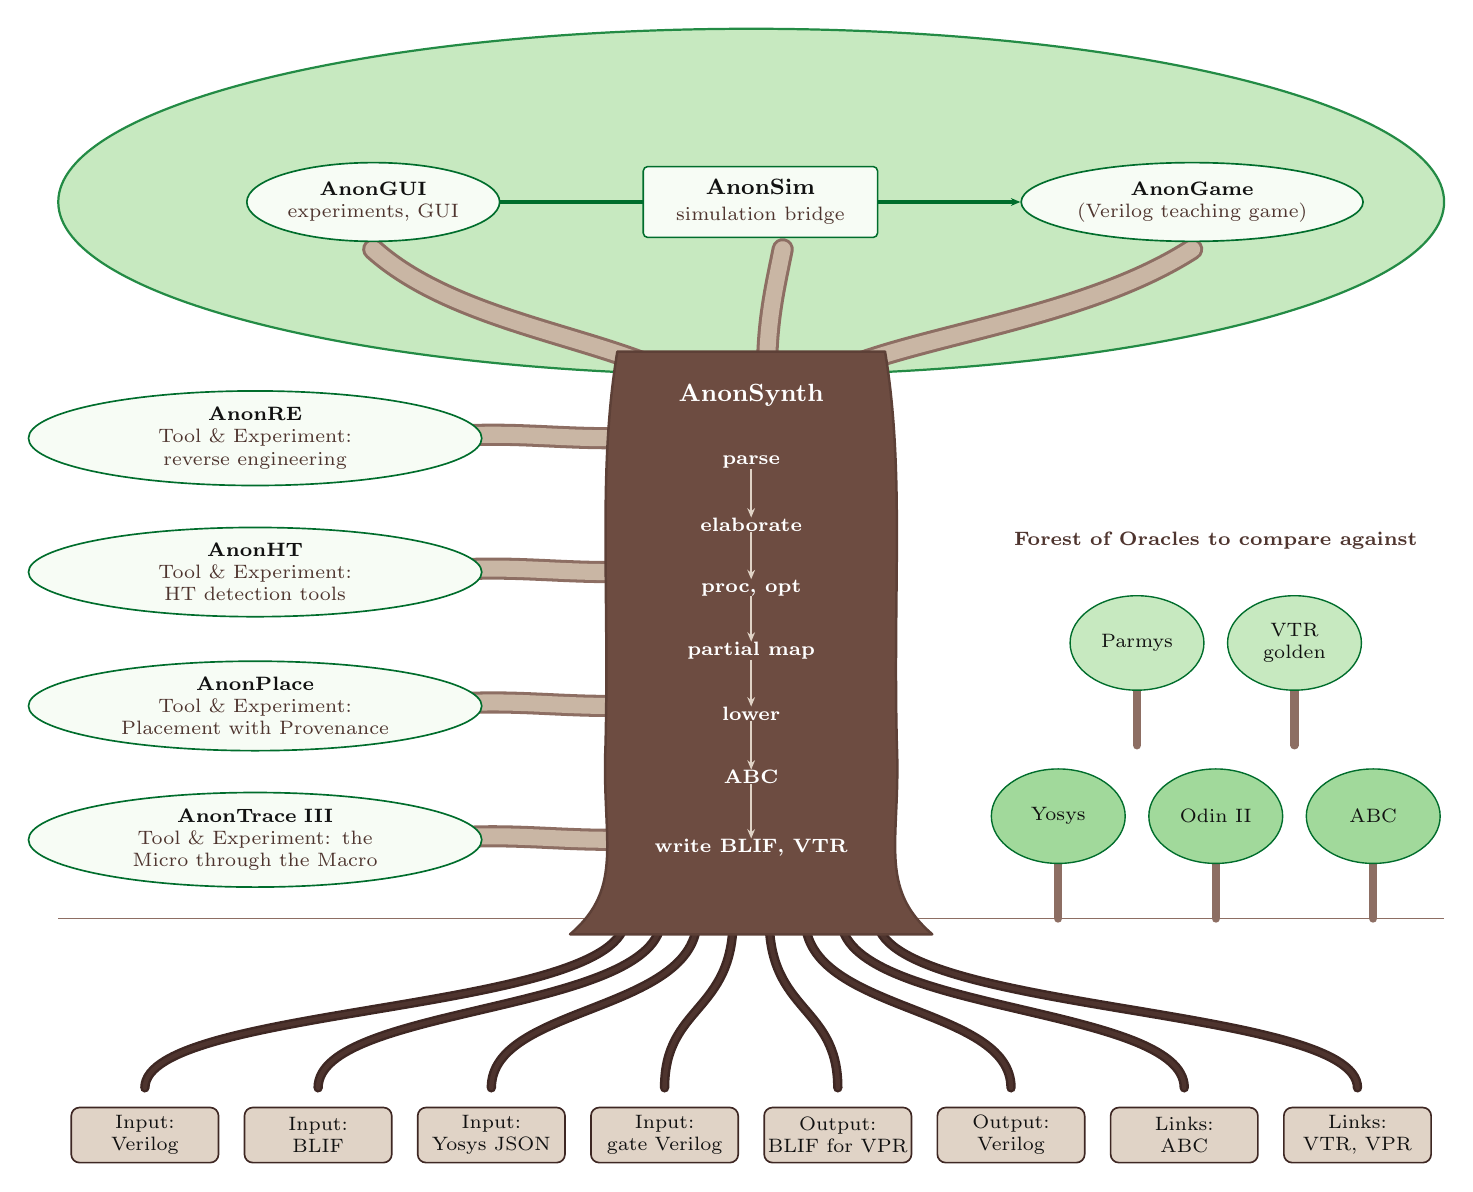
\begin{tikzpicture}[odin, node distance=3mm,
  leaf/.style={ellipse, draw=o3grn8, fill=o3grn1, align=center, line width=0.6pt, inner xsep=1pt,
               inner ysep=1pt, minimum width=15mm, minimum height=8.5mm, font=\scriptsize},
  tip/.style={rectangle, rounded corners=3pt, draw=o3brn9, fill=o3brn3, align=center, line width=0.6pt, inner xsep=1pt,
              inner ysep=1pt, minimum height=7mm, font=\scriptsize},
  limb/.style={line width=8pt, draw=o3brn5, line cap=round},
  limbin/.style={line width=5.8pt, draw=o3brn4, line cap=round},
  rootl/.style={line width=3.4pt, draw=o3brn9, line cap=round},
  rootin/.style={line width=1.6pt, draw=o3brn7, line cap=round},
  stp/.style={font=\scriptsize\bfseries, text=white, inner sep=0pt, align=center},
  mini/.style={ellipse, draw=o3grn8, fill=o3grn3, line width=0.5pt, align=center, inner sep=0pt,
               minimum width=17mm, minimum height=12mm, font=\scriptsize}]
  % ---- roots (drawn first, behind the trunk) ----------------------------------------------
  \foreach \i/\t in {0/Input:\\Verilog, 1/Input:\\BLIF, 2/Input:\\Yosys JSON, 3/Input:\\gate Verilog,
                     4/Output:\\BLIF for VPR, 5/Output:\\Verilog, 6/Links:\\ABC, 7/{Links:\\VTR, VPR}}{
    \pgfmathsetmacro{\x}{-7.7+2.2*\i}
    \pgfmathsetmacro{\tx}{-1.6+0.457*\i}
    \draw[rootl]  (\tx,0.3) .. controls (\tx,-0.9) and (\x,-0.8) .. (\x,-1.85);
    \draw[rootin] (\tx,0.3) .. controls (\tx,-0.9) and (\x,-0.8) .. (\x,-1.85);
    \node[tip, text width=18mm] at (\x,-2.45) {\t};
  }
  % ---- ground line ---------------------------------------------------------------------
  \draw[o3brn5, line width=0.6pt] (-8.8,0.3) -- (8.8,0.3);
  % ---- the oracle forest: two rows of mini trees, no overlaps ----------------------------------
  \foreach \x/\y/\t/\c in {4.9/2.5/Parmys/o3grn3, 6.9/2.5/{VTR\\golden}/o3grn3,
                            3.9/0.3/Yosys/o3grn4, 5.9/0.3/{Odin~II}/o3grn4, 7.9/0.3/ABC/o3grn4}{
    \draw[line width=3pt, draw=o3brn5, line cap=round] (\x,\y) -- (\x,\y+0.75);
    \node[mini, fill=\c] at (\x,\y+1.3) {\t};
  }
  \node[regionlabel] at (5.9,5.1) {Forest of Oracles to compare against};
  % ---- canopy: the oval is the tree-top (low) ------------------------------------------------
  \node[ellipse, fill=o3grn3, draw=o3grn7, line width=0.8pt, minimum width=176mm,
        minimum height=44mm, inner sep=0pt] at (0,9.4) {};
  % ---- limbs to the canopy pieces (behind the trunk) --------------------------------------------
  \draw[limb]   (-1.0,7.2) .. controls (-2.0,7.7) and (-3.8,7.9) .. (-4.8,8.8);
  \draw[limbin] (-1.0,7.2) .. controls (-2.0,7.7) and (-3.8,7.9) .. (-4.8,8.8);
  \draw[limb]   (1.0,7.2) .. controls (2.0,7.7) and (4.2,7.9) .. (5.6,8.8);
  \draw[limbin] (1.0,7.2) .. controls (2.0,7.7) and (4.2,7.9) .. (5.6,8.8);
  \draw[limb]   (0.2,7.2) .. controls (0.2,7.9) and (0.3,8.3) .. (0.4,8.8);
  \draw[limbin] (0.2,7.2) .. controls (0.2,7.9) and (0.3,8.3) .. (0.4,8.8);
  % ---- side branches off the trunk: tools and experiments ---------------------------------------
  \foreach \y in {6.4, 4.7, 3.0, 1.3}{
    \draw[limb]   (-1.8,\y) .. controls (-2.6,\y) and (-3.2,\y+0.1) .. (-4.1,\y);
    \draw[limbin] (-1.8,\y) .. controls (-2.6,\y) and (-3.2,\y+0.1) .. (-4.1,\y);
  }
  % ---- trunk: AnonSynth on top, its steps going down to the roots --------------------------------
  \path[draw=o3brn8, fill=o3brn6, line width=0.9pt]
    (-2.3,0.1) .. controls (-1.6,0.7) and (-1.9,1.3) .. (-1.85,2.5)
    .. controls (-1.8,4.5) and (-1.95,6.0) .. (-1.7,7.5)
    -- (1.7,7.5) .. controls (1.95,6.0) and (1.8,4.5) .. (1.85,2.5)
    .. controls (1.9,1.3) and (1.6,0.7) .. (2.3,0.1) -- cycle;
  \node[font=\small\bfseries, text=white] at (0,6.95) {AnonSynth};
  \foreach \y/\t [count=\i] in {6.1/parse, 5.3/elaborate, 4.5/{proc, opt}, 3.7/partial map,
                                2.9/lower, 2.1/ABC, 1.2/{write BLIF, VTR}}{
    \node[stp] (st\i) at (0,\y) {\t};
  }
  \foreach \a/\b in {1/2, 2/3, 3/4, 4/5, 5/6, 6/7}{
    \draw[->, draw=o3brn3, line width=0.5pt] (st\a.south) -- (st\b.north);
  }
  % ---- canopy pieces ----------------------------------------------------------------------------
  \node[leaf, text width=22mm, minimum height=10mm] (wyrd) at (-4.8,9.4) {\textbf{AnonGUI}\\\odinsub{experiments, GUI}};
  \node[leaf, text width=30mm, minimum height=10mm] (mid) at (5.6,9.4) {\textbf{AnonGame}\\\odinsub{(Verilog teaching game)}};
  \draw[->, line width=1.6pt, draw=o3grn8] (wyrd.east) -- (mid.west)
    node[pos=0.5, box, draw=o3grn8, fill=o3grn1, text width=28mm, minimum height=9mm] {\textbf{AnonSim}\\\odinsub{simulation bridge}};
  % ---- tools and experiments on side branches ---------------------------------------------------------
  \node[leaf, text width=40mm, minimum height=11mm] (lok) at (-6.3,6.4) {\textbf{AnonRE}\\\odinsub{Tool \& Experiment: reverse engineering}};
  \node[leaf, text width=40mm, minimum height=11mm] (lr)  at (-6.3,4.7) {\textbf{AnonHT}\\\odinsub{Tool \& Experiment: HT detection tools}};
  \node[leaf, text width=40mm, minimum height=11mm] (nor) at (-6.3,3.0) {\textbf{AnonPlace}\\\odinsub{Tool \& Experiment: Placement with Provenance}};
  \node[leaf, text width=40mm, minimum height=11mm] (ver) at (-6.3,1.3) {\textbf{AnonTrace~III}\\\odinsub{Tool \& Experiment: the Micro through the Macro}};
\end{tikzpicture}
}}
\caption{AnonSuite drawn as a tree. The roots are the inputs and the tools AnonSynth links to. The trunk is AnonSynth, with its steps. The oracles are the small forest beside it. Three wells hold outside work. The canopy holds AnonGUI, AnonSim, AnonGame (a Verilog teaching game~\cite{anon02}) and the fruit, AnonData. Side branches: AnonRE, AnonHT, AnonPlace (placement~\cite{anon05}) and AnonTrace~III.}
\label{fig:yggdrasil}
\end{figure*}

% ------------------------------------------------------------------------------------------
\section{Background}
\label{sec:background}

\subsection{Glossary}
\label{sec:glossary}

Terms in dependency order: each uses only terms above it. The definitions of the basic FPGA and CAD terms follow the order and the wording of the thesis on heterogeneous FPGAs and of the thesis on architecture-aware packing and VTR~\cite{luuthesis}; the others describe AnonSynth and its checks.

\begingroup\small
\par\noindent\textbf{FPGA.} A chip of programmable logic blocks and wires onto which a digital design is loaded. % ref:fpga
\par\noindent\textbf{flip-flop.} A one-bit storage cell that keeps its value between clock edges. % ref:ff
\par\noindent\textbf{LUT.} Look-up table: a small memory that implements any logic function of $K$ inputs ($K=6$ here). A LUT and a flip-flop form the basic logic element of most FPGAs. % ref:lut
\par\noindent\textbf{CLB.} Configurable logic block: a group of LUTs and flip-flops that is placed as one unit (a cluster)~\cite{luuthesis}. % ref:clb
\par\noindent\textbf{Verilog / HDL.} The hardware description language (HDL) in which a designer writes a circuit; Verilog is the one used here. % ref:hdl
\par\noindent\textbf{netlist.} The list of the gates, LUTs and other cells of a design and the wires (nets) between them. % ref:netlist
\par\noindent\textbf{synthesis front end.} The program that reads the HDL and produces a netlist for the rest of the flow. % ref:front
\par\noindent\textbf{elaboration.} The first step of a front end: turn the parsed HDL into a design graph by resolving parameters, generate loops and hierarchy. % ref:elab
\par\noindent\textbf{ABC.} The logic-synthesis program that maps the gates of a netlist onto LUTs (technology mapping). % ref:abc
\par\noindent\textbf{packing, placement, routing.} Packing groups LUTs and flip-flops into CLBs; placement chooses a site on the chip for each CLB; routing chooses the wires between them. % ref:prp
\par\noindent\textbf{VTR / VPR.} The open-source FPGA CAD flow (Verilog-to-Routing, VTR) and its packing, placement and routing program (VPR)~\cite{luuthesis}. % ref:vtr
\par\noindent\textbf{Odin II / Yosys / Parmys.} Odin II was the front end of VTR; Yosys is an open synthesis tool and Parmys the Yosys plugin that now serves VTR as its front end. % ref:odin2
\par\noindent\textbf{provenance.} The link from each netlist object back to the HDL that produced it. % ref:prov
\par\noindent\textbf{Dark Factory.} A software process in which agents turn a human's specification into software, with no human writing the code. % ref:dark
\par\noindent\textbf{channel width.} The number of routing tracks in each channel that the router needs to route a design (minimum channel width $W$)~\cite{luuthesis}. % ref:minw
\par\noindent\textbf{wirelength.} The total length of the wires a routed design uses. % ref:wl
\par\noindent\textbf{critical path / CPD.} The slowest path between registers and its delay in ns (critical-path delay, CPD)~\cite{luuthesis}. % ref:cpd
\par\noindent\textbf{near-critical.} A path whose delay is within a stated window of the critical-path delay. % ref:near
\par\noindent\textbf{area.} How much chip a design uses: the number of LUTs, the number of CLBs and the minimum channel width $W$. % ref:area
\par\noindent\textbf{speed.} How fast the circuit runs: the critical-path delay and the routed wirelength, and where available the near-critical paths. % ref:speed
\par\noindent\textbf{power.} The energy the circuit uses. This paper does not measure it. % ref:power
\par\noindent\textbf{hypothesis / verdict.} A hypothesis is a claim that an experiment can confirm or fail to confirm. The verdict is USEFUL (confirmed under the stated gate or check), POSSIBLY GOOD (confirmed but narrow or fragile), INCONCLUSIVE (neither confirmed nor failed) or DISMISSED (failed). % ref:hyp
\par\noindent\textbf{IR.} Intermediate representation: AnonSynth's one internal design graph, with a view of multi-bit words and a view of single bits. % ref:ir
\par\noindent\textbf{oracle.} A trusted reference tool whose output we compare against (Yosys with Parmys, and Odin II). % ref:oracle
\par\noindent\textbf{C ABI / plugin.} The application binary interface (ABI) is the stable C interface through which a plugin, a separately built program that adds passes or cell types, and AI tools drive AnonSynth without changing it. % ref:abi
\par\noindent\textbf{AST.} Abstract syntax tree: the parsed form of the HDL text. % def:ast
\par\noindent\textbf{golden.} The stored result of an oracle for a design, kept so that later runs compare against it. % def:golden
\par\noindent\textbf{partial mapping.} Binding the parts of a design that fit the architecture's dedicated blocks (multipliers, adders, memories) to those blocks and leaving the rest as gates for ABC. % def:pmap
\par\noindent\textbf{word cell / bit cell / lower.} A word cell is a multi-bit operator in the IR; a bit cell is a one-bit gate; the pass lower turns word cells into bit cells. % def:word
\par\noindent\textbf{proc, opt, fsm, wreduce, flatten.} The word-level passes re-implemented from Yosys 0.55: processes to multiplexers and flip-flops; clean-up; state-machine recoding; width reduction; inlining of the hierarchy. % def:passes
\par\noindent\textbf{BLIF.} The netlist text format that VPR reads. % def:blif
\par\noindent\textbf{lineage DAG.} The append-only graph of source, imported and derived records, with labelled joins, that sits behind each provenance ID. % def:lineage
\par\noindent\textbf{geomean ratio.} The geometric mean over designs of the ratio AnonSynth over Parmys; 1.0 means equal and below 1.0 is better for area and delay. % def:geomean
\par\noindent\textbf{leg (P, O, O$'$).} One run of the quality-of-results harness: P is the Parmys flow (the baseline), O is AnonSynth with its linked ABC, and O$'$ is AnonSynth's netlist through VTR's own ABC stage. % def:leg
\par\noindent\textbf{QoR gate.} The acceptance bound on quality of results: geomean ratio at most 1.20 and no design above 1.50 on the gated metrics. % def:gate
\par\noindent\textbf{equivalence (SAT, refinement).} A proof, by SAT, that two designs give the same outputs, or that one refines the other; unproven when the design is past the size limit of the solver. % def:equiv
\par\noindent\textbf{fcheck (functional check).} VTR's random check: build the RTL and the netlist with Verilator and drive both with 50,000 random vectors. % def:fcheck
\par\noindent\textbf{determinism.} Rerunning gives byte-identical output. % def:det
\par\noindent\textbf{exit-code discipline.} A list of expected differences never turns an unproven result into a pass; tools report 0 holds, 1 differs, 2 tool error, 3 hard failure, 4 unproven, 77 skipped. % def:exit
\endgroup

\subsection{Two open-source models of Verilog synthesis}

\emph{The Odin~II flow.} Odin~II~\cite{jamieson2011odin2} parses Verilog with Bison and Flex into an abstract syntax tree (AST); passes over the AST and the module hierarchy turn it into one flattened netlist of nodes, pins, and nets. It reads the VPR architecture file to decide which multipliers, adders, and memories become dedicated blocks, writes the rest as BLIF for ABC~\cite{brayton2010abc} to map to LUTs, and includes a netlist simulator.

\emph{The Yosys approach.} Yosys~\cite{wolf2013yosys} parses Verilog into an AST, and \code{genrtlil} turns each module into RTLIL, a word-level netlist of wires, cells, processes and memories, with the hierarchy kept. From then on, every step is a pass over RTLIL that never sees the AST: \code{proc}, the \code{opt} family, \code{flatten}, \code{techmap} and \code{abc}. Yosys is the reference open synthesis suite, with a large pass library and SystemVerilog and VHDL through plugins~\cite{yosysslang,ghdl}.

\subsection{VTR and partial mapping}

Both models attach to VTR~\cite{luu2009vpr5,rose2012vtr,luu2014vtr7,murray2020vtr8}: a front end, ABC, then VPR's packing, placement, and routing on an XML-described architecture. Jason Luu's work brought in partial mapping. His architecture description language~\cite{luu2011packing} describes logic blocks with hierarchy, modes, and complex interconnects, and models each dedicated block's primitive, so a front end that reads the same file can map part of a design onto those blocks and leave the rest soft for ABC. VTR~7.0~\cite{luu2014vtr7} and the study of hard adders and carry chains~\cite{luu2014hardadders} carried this to adders, with front-end optimizations that ease the restrictions hardened arithmetic places on logic synthesis. Parmys~\cite{parmys} brings the same partial mapping onto Yosys's word-level netlists, runs inside VTR's pinned Yosys~0.55, and is now VTR's default front end.

\subsection{The provenance problem}
\label{sec:provenance-problem}

Synthesis modifies some of the designer's functional intention. Flattening removes the hierarchy, optimization merges and splits operators, and LUT mapping covers the logic with cells that have no source line names. I call the task of linking each object of the final netlist back to the HDL that produced it the \emph{provenance problem}; it is one of the major pieces of this work going forward. Earlier work addressed it in placement: simulated annealing produces a flattened design that loses its HDL hierarchy, so they recovered system-level information from the flat netlist and analyzed its correlation with locality in FPGA placement~\cite{anon04,anon05}, then identified and placed clusters found in the placement data~\cite{anon06}. Later work applies data-mining clustering to such combinatorial optimization algorithms~\cite{anon07}. Goeders and Wilton address the same problem in in-system debug: signals in a high-level synthesis-built circuit must be traced back to their source, and they developed signal-tracing and debug techniques for such circuits on FPGAs~\cite{goeders2014effective,goeders2015dynamic,goeders2017signaltracing}. Each line of work had to recover a link the synthesis tool didn't keep. AnonSynth keeps it (Sec.~\ref{sec:arch}), so its analysis flow (provenance coverage, \code{levelize}, graph export) can redo the placement-correlation experiment with the link to the HDL measured rather than recovered.

\subsection{Oracles, ASTs and elaboration}

\code{tools/run-oracle.sh} runs an oracle on a design and an architecture and stores its netlist, logs, and commit as a golden; AnonSynth's output is compared with the golden for identity after canonical renaming and for functional equivalence. An oracle is trusted because it is the reference, not because it is always right (Sec.~\ref{sec:parmys-bugs}). Odin~II transforms the AST into one flat netlist, while Yosys builds each module separately and flattens later as a pass on the graph; AnonSynth takes the RTLIL route with its own split (Sec.~\ref{sec:arch}).  We note that an oracle makes the process much simpler than the original creation of Odin and Odin~II, which humans verified at high cost.

% ------------------------------------------------------------------------------------------
\section{The Innovations}
\label{sec:arch}

Each subsection gives the innovation in plain English first and the technical description second. The experiments that test them are in Sec.~\ref{sec:results}.

\subsection{A front end that plugs into VTR}
\label{sec:vtr-link}

\emph{Plain English.} AnonSynth reads Verilog, makes a netlist, and hands it to ABC and VPR as before. Plugging into VTR is not the real goal of AnonSynth; it is the proof that each step works on real designs, because VTR comes with golden results to compare with. The result is meant to be comparable with the Yosys-based front end, not equal to it.

\begin{figure*}[t]
\centering
\odinfit{\textwidth}{% The AnonSynth flow with what each stage does (see fig_flow_base.tex). Wide: \textwidth.
\def\flowbandA{Verilog files, include paths, defines, top, parameters, and the architecture and
  rules: one project record.}%
\def\flowbandB{Preprocessor with a segment map; Bison/Flex parser builds the AST; the symbol
  table maps each name to its declaration, per scope.}%
\def\flowbandC{None. Stage 1 of elaboration evaluates parameters, \odintt{generate} and constant
  functions, because the language requires it. The script runs no \odintt{opt} before \odintt{proc}.}%
\def\flowbandD{Stage 1: elaborated AST (the seam). Stage 2: bind names, widths, word cells;
  \odintt{always} becomes a \odintt{\$proc} cell. \odintt{proc}: muxes, latches, flip-flops.}%
\def\flowbandE{\odintt{fsm}: find and recode state machines. \odintt{opt}: \odintt{opt\_expr}
  folds constants; \odintt{opt\_clean} removes dead cells; \odintt{opt\_merge} merges equal cells;
  \odintt{opt\_share} shares operators. \odintt{flatten}: inline instances. \odintt{wreduce}: narrow widths.}%
\def\flowbandF{Binds \odintt{\$mul}, \odintt{\$add}/\odintt{\$sub} and \odintt{\$mem} to the hard
  blocks the arch record lists: multipliers, adder chains, RAM. The rest stays soft.}%
\def\flowbandG{Every word cell becomes bit cells; flip-flops become \odintt{\$\_DFF\_P\_}; a
  leftover \odintt{\$mem} becomes flip-flops and muxes.}%
\def\flowbandH{Linked ABC optimises the soft logic as an AIG and maps it to $K$-input LUTs,
  one run per clock domain. Hard cells are cut points.}%
\def\flowbandI{BLIF \odintt{--vtr} for VPR; structural Verilog; Yosys JSON; LPM Verilog for
  Quartus; Graphviz \odintt{dot}; RTLIL to Yosys.}%
\def\flowbandJ{Each output can be read back with its HDL locations: \odintt{read\_blif},
  \odintt{read\_verilog -icells}, \odintt{read\_json}.}%
% The AnonSynth flow, drawn once (the O leg of tools/vtr-qor, qor_legs.py, plus the readers of
% Phase 5). Nine stages in two rows, a band of text under each box. The three figures that use it
% (fig_flow, fig_flow_verify, fig_flow_prov) define \flowbandA ... \flowbandJ, the text of each
% band, and then input this file. Wide figure: \textwidth.
\begin{tikzpicture}[odin,
  st/.style={box, light, text width=29.5mm, minimum height=13mm, inner ysep=2pt},
  band/.style={font=\scriptsize, text width=29.5mm, align=left, anchor=north, inner sep=1.2pt,
               color=o3ink}]
  % ---- row 1 ---------------------------------------------------------------------------
  \node[st] (s1) at (0, 0) {\textbf{Code}\\[-1pt]\odinsub{Verilog and the project}};
  \node[st] (s2) at (3.4, 0) {\textbf{Parse}\\[-1pt]\odinsub{\odintt{read\_verilog}: AST and symbol table}};
  \node[st, light] (s3) at (6.8, 0) {\textbf{Before elaboration}\\[-1pt]\odinsub{no optimisation pass}};
  \node[st] (s4) at (10.2, 0) {\textbf{Elaborate}\\[-1pt]\odinsub{stage 1, stage 2, \odintt{proc}}};
  \node[st] (s5) at (13.6, 0) {\textbf{Word-level passes}\\[-1pt]\odinsub{\odintt{fsm}, \odintt{opt}, \odintt{flatten}, \odintt{wreduce}}};
  % ---- row 2 ---------------------------------------------------------------------------
  \node[st] (s6) at (0, -5.4) {\textbf{Partial mapping}\\[-1pt]\odinsub{\odintt{partial\_map} (\odintt{hardmap}) on the arch record}};
  \node[st] (s7) at (3.4, -5.4) {\textbf{Lower}\\[-1pt]\odinsub{\odintt{lower}: words to bits}};
  \node[st] (s8) at (6.8, -5.4) {\textbf{Logic and LUTs}\\[-1pt]\odinsub{linked ABC: \odintt{abc --lut K}}};
  \node[st] (s9) at (10.2, -5.4) {\textbf{Outputs}\\[-1pt]\odinsub{\odintt{write\_blif --vtr}, Verilog, JSON, LPM, dot}};
  \node[st, light] (s10) at (13.6, -5.4) {\textbf{Read back}\\[-1pt]\odinsub{BLIF, Verilog, JSON readers (Phase 5)}};
  % ---- bands ---------------------------------------------------------------------------
  \foreach \i/\t in {1/\flowbandA, 2/\flowbandB, 3/\flowbandC, 4/\flowbandD, 5/\flowbandE,
                     6/\flowbandF, 7/\flowbandG, 8/\flowbandH, 9/\flowbandI, 10/\flowbandJ}
    \node[band] at ([yshift=-1.4mm]s\i.south) {\t};
  % ---- edges ---------------------------------------------------------------------------
  \foreach \a/\b in {s1/s2, s2/s3, s3/s4, s4/s5, s6/s7, s7/s8, s8/s9}
    \draw[flow] (\a) -- (\b);
  \draw[flow] (s5.east) -- ++(0.4,0) |- (0,-4.4) -- (s6.north);
  \draw[ref] (s9) -- (s10);
\end{tikzpicture}

}
\caption{The flow of a Verilog design through AnonSynth, in the order of the production script. Each box is a stage; the text under it says what it does. Every stage from \code{proc} to \code{write\_blif} is a registered pass.}
\label{fig:flow}
\end{figure*}

\emph{Technical.} AnonSynth reads a design into one IR and changes it one pass at a time. Figure~\ref{fig:flow} shows the path of a Verilog design through the stages, in the order of the production script:
\emph{One IR, two views.} Each cell type carries a granularity tag (\code{word}, \code{bit}, \code{hard}, \code{blackbox}); the word-level (RTLIL) and bit-level (netlist) views are assertions over that tag, so every reader, writer, checker, and the simulator exist once. Every net is one bit, ports are nodes, constants are cells, and every reference is a typed 32-bit ID into per-module paged storage, never a pointer. Every reader, writer, and transformation is a pass, and in Debug builds the pass manager runs a structural \code{check} before and after each.

\emph{Elaboration in two stages.} A project record names the files, the top, the parameters and, unusually for a front end, the architecture and the mapping rules. A preprocessor and an LALR(1) parser build an AST with source locations. Stage~1 is Verilog-specific: it resolves parameters, \code{generate} and constant functions into an \emph{elaborated AST}. Stage~2 is language-neutral: it binds names, sizes expressions, and builds word-level cells, keeping each \code{always} block as a \code{\$proc} cell. The seam lets a later front end enter at stage~2.

\emph{Word-level passes.} \code{proc} lowers \code{\$proc} cells to multiplexer trees, latches and flip-flops in Yosys~0.55's order, and \code{fsm} recodes state machines where Parmys does. \code{opt} is Yosys's family of rewrites, \code{flatten} inlines instances top-down keeping each object's instance path, and \code{wreduce} narrows widths, which decides the block counts. Every walk that Yosys writes recursively is an explicit worklist here, and every input-driven quantity has a named cap, so a hostile input gives a located error, not a crash.

\emph{Partial mapping.} \code{partial\_map} (script name \code{hardmap}) binds word-level multipliers, adders, and RAMs to the blocks that the architecture lists and leaves the rest soft. Parmys's rule is the default; \code{read\_arch} fills a tech library, and an arch record from a VPR architecture file, and generic blocks match by exact port signature, as in Odin~II.

\emph{Bits, LUTs and BLIF.} \code{lower} turns every remaining word cell into bit cells. \code{abc} runs a linked ABC once per clock domain and returns LUTs as one registry cell, \code{\$lut}, with VTR's own script as the default (other scripts are allow-listed and run in a child process). \code{write\_blif --vtr} writes the top module as BLIF that VPR reads; it refuses, before any byte is written, every construct VPR would reject, and \code{blif-vtr-check} mirrors VPR's BLIF checks so that CI gets VPR's verdicts without VTR. The QoR harness \code{vtr-qor} runs VTR's own scripts, read-only, in legs that separate the causes of a gap. Where AnonSynth and Parmys could differ, \code{--vtr-compat} makes AnonSynth do what Parmys does and print a WARNING; where Parmys is wrong to the RTL, AnonSynth stays correct and declares the difference (Sec.~\ref{sec:parmys-bugs}).

\subsection{Checking against oracles}

\emph{Plain English.} Every stage of AnonSynth is checked by a tool that is separate from the code, against a reference. Where AnonSynth and the reference differ, a probe decides which one matches the Verilog, so the reference's own mistakes surface, and an unproven result never counts as a pass.

\emph{Technical.} Figure~\ref{fig:flow-verify} marks which technique checks which stage: refinement proofs by SAT (\code{lower-equiv}, \code{opt-equiv}), random module generators checked against Yosys \code{techmap}, Verilator random vectors (\code{fcheck}), golden BLIFs, and the exit-code convention of Sec.~\ref{sec:abi-summary}.

\subsection{One provenance-tracked IR}

\begin{figure}[t]
\centering
\odinfit{\columnwidth}{% Provenance lineage DAG (IR-12, IR-13), an illustrative example: one source line inside a
% generate loop elaborates to two $add cells (two SOURCE records, told apart by hier path);
% lowering each $add is one operation (one DERIVED record shared by its pieces); merging two
% gates is one operation with two parents. Records are immutable, hash-consed and design-wide;
% parents always have smaller IDs. Run and op numbers are illustrative. Single column.
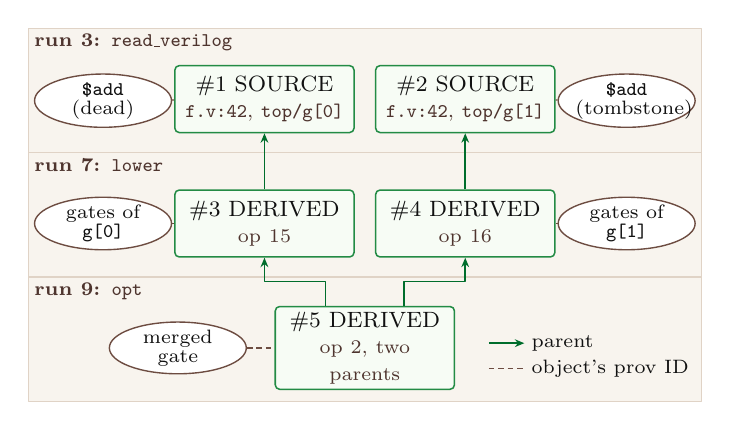
\begin{tikzpicture}[odin,
  rec/.style={box, light, text width=21mm, minimum height=8.5mm},
  obj/.style={ellipse, draw=o3brn6, fill=white, line width=0.5pt, font=\scriptsize,
              align=center, inner xsep=-1pt, inner ysep=0pt, minimum height=6mm, text width=13mm},
  parent/.style={flow, draw=o3grn8},
  pid/.style={line width=0.5pt, draw=o3brn6, dash pattern=on 2pt off 1.4pt},
  band/.style={fill=o3brn1, draw=o3brn3, line width=0.4pt},
  bandlabel/.style={font=\scriptsize\bfseries, color=o3brn7, anchor=north west, inner sep=2pt}]
  % ---- run bands ---------------------------------------------------------------------------
  \foreach \y/\t in {0/{run 3: \odintt{read\_verilog}}, -1.58/{run 7: \odintt{lower}},
                     -3.16/{run 9: \odintt{opt}}} {
    \fill[band] (0, \y+0.72) rectangle (8.55, \y-0.86);
    \node[bandlabel] at (0, \y+0.72) {\t};
  }
  % ---- records -----------------------------------------------------------------------------
  \node[rec] (r1) at (3.0, -0.18)  {\#1 SOURCE\\\odinsub{\odintt{f.v:42}, \odintt{top/g[0]}}};
  \node[rec] (r2) at (5.55, -0.18)  {\#2 SOURCE\\\odinsub{\odintt{f.v:42}, \odintt{top/g[1]}}};
  \node[rec] (r3) at (3.0, -1.76) {\#3 DERIVED\\\odinsub{op 15}};
  \node[rec] (r4) at (5.55, -1.76) {\#4 DERIVED\\\odinsub{op 16}};
  \node[rec] (r5) at (4.275, -3.34) {\#5 DERIVED\\\odinsub{op 2, two parents}};
  % ---- IR objects --------------------------------------------------------------------------
  \node[obj] (a1) at (0.95, -0.2) {\odintt{\$add}\\[-1pt](dead)};
  \node[obj] (a2) at (7.6, -0.2) {\odintt{\$add}\\[-1pt](tombstone)};
  \node[obj] (g1) at (0.95, -1.76) {gates of\\[-1pt]\odintt{g[0]}};
  \node[obj] (g2) at (7.6, -1.76) {gates of\\[-1pt]\odintt{g[1]}};
  \node[obj] (g3) at (1.9, -3.34) {merged\\[-1pt]gate};
  % ---- edges -------------------------------------------------------------------------------
  \draw[parent] (r3) -- (r1);
  \draw[parent] (r4) -- (r2);
  \draw[parent] (r5.north) ++(-0.5,0) |- ($(r3.south)+(0,-0.3)$) -- (r3.south);
  \draw[parent] (r5.north) ++(0.5,0) |- ($(r4.south)+(0,-0.3)$) -- (r4.south);
  \foreach \o/\r in {a1/r1, a2/r2, g1/r3, g2/r4, g3/r5} \draw[pid] (\o) -- (\r);
  % ---- key ---------------------------------------------------------------------------------
  \begin{scope}[shift={(5.85, -3.6)}]
    \draw[parent] (0, 0.32) -- (0.45, 0.32);
    \node[font=\scriptsize, anchor=west, inner sep=1pt] at (0.5, 0.32) {parent};
    \draw[pid] (0, 0) -- (0.45, 0);
    \node[font=\scriptsize, anchor=west, inner sep=1pt] at (0.5, 0) {object's prov ID};
  \end{scope}
\end{tikzpicture}
}
\caption{The provenance lineage DAG (illustrative run and operation numbers). Two \code{\$add}s from one line of a generate loop get two SOURCE records; lowering each is one operation with one DERIVED record; clumping two gates is one operation with two parents.}
\label{fig:prov}
\end{figure}

\emph{Plain English.} Every object in the netlist remembers which Verilog text made it, and from v1.2.0 it remembers the full chain of constructs, including the places where two constructs were blended. This is AnonSynth's answer to the provenance problem (Sec.~\ref{sec:provenance-problem}) and the property the AnonData dataset rests on.

\emph{Technical.} Every node, net and wire carries one 32-bit ID into an append-only lineage DAG (Fig.~\ref{fig:prov}). A record is SOURCE (made from the HDL), IMPORTED (read from a netlist) or DERIVED (made by a pass, with its parents), and it holds the pass run and the operation within it, so 100 adders from one line of a generate loop stay distinguishable. A step that blends constructs is labelled a join. The walk runs backward to the source line and forward from \code{file:line}, and the writers can name each object \code{hier/path/name@file:line}, so a VPR block traces to its source line without AnonSynth loaded. v1.2.0 adds the construct table (ABI~7) and a version~2 name map, which \code{names --lookup} and \code{names --chain} read and \code{anonsynth-prov-post} extends after place and route.

\subsection{The ABI: extensions and AI tools}
\label{sec:abi-summary}

\begin{figure}[t]
\centering
\odinfit{\columnwidth}{% The C ABI and plugin model (1D spec, DESIGN.md section 15.3, include/anonsynth/anonsynth.h ABI v4).
% Everything outside the core sees only anonsynth.h. Single column: \columnwidth.
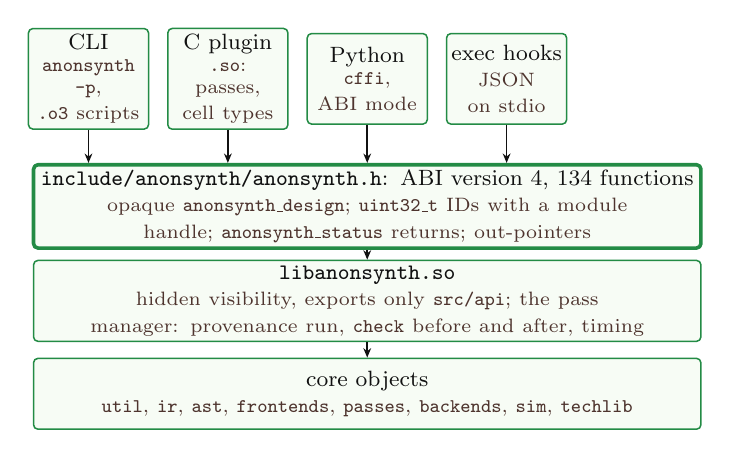
\begin{tikzpicture}[odin,
  client/.style={box, text width=14.2mm, minimum height=11.5mm, inner xsep=1.5pt},
  layer/.style={box, text width=83mm, minimum height=9mm}]
  % ---- clients -------------------------------------------------------------------------------
  \foreach \n/\x/\s/\t/\u in {
      cli/0.83/light/{CLI}/{\odintt{anonsynth -p},\\\odintt{.o3} scripts},
      so/2.6/light/{C plugin}/{\odintt{.so}: passes,\\cell types},
      py/4.37/light/{Python}/{\odintt{cffi},\\ABI mode},
      hook/6.14/light/{exec hooks}/{JSON on stdio}}
    \node[client, \s] (\n) at (\x, 0) {\t\\\odinsub{\u}};
  % ---- layers --------------------------------------------------------------------------------
  \node[layer, light, emph] (hdr) at (4.37, -1.62)
       {\odintt{include/anonsynth/anonsynth.h}: ABI version 4, 134 functions\\
        \odinsub{opaque \odintt{anonsynth\_design}; \odintt{uint32\_t} IDs with a module handle;
                 \odintt{anonsynth\_status} returns; out-pointers}};
  \node[layer, light] (lib) at (4.37, -2.82)
       {\odintt{libanonsynth.so}\\
        \odinsub{hidden visibility, exports only \odintt{src/api}; the pass manager: provenance
                 run, \odintt{check} before and after, timing}};
  \node[layer, light] (core) at (4.37, -4.0)
       {core objects\\
        \odinsub{\odintt{util}, \odintt{ir}, \odintt{ast}, \odintt{frontends}, \odintt{passes},
                 \odintt{backends}, \odintt{sim}, \odintt{techlib}}};
  % ---- edges ---------------------------------------------------------------------------------
  \foreach \n in {cli, so, py} \draw[flow] (\n.south) -- (\n.south |- hdr.north);
  \foreach \n in {hook}    \draw[flow] (\n.south) -- (\n.south |- hdr.north);
  \draw[flow] (hdr) -- (lib);
  \draw[flow] (lib) -- (core);
\end{tikzpicture}
}
\caption{The C ABI and plugin model. Everything outside the core sees only \code{anonsynth.h}.}
\label{fig:abi}
\end{figure}

\emph{Plain English.} Other programs of the suite can drive and read AnonSynth through one stable interface, and AI tools attach the same way.

\emph{Technical.} The interface is the contract between compiled code: function names, types, structure layouts, and calling conventions. A plugin built against one version of AnonSynth must load against a later build without a recompile, and a C ABI helps: no name mangling, no class layouts, no exceptions across the boundary, and other languages can call it. \code{include/anonsynth/anonsynth.h} is the only header a plugin sees (Fig.~\ref{fig:abi}). The ABI version (7 at v1.2.0) exposes an opaque design handle and raw 32-bit IDs; every function returns a status; \code{libanonsynth.so} exports only what the header declares (a script checks it), and a plugin that asks for another ABI version is refused. Plugins register passes and cell types from an \code{anonsynth\_plugin\_init} entry point, and Python uses the same header through cffi.

The same boundary is how AI tools attach. Agents built AnonSynth by driving its command-line scripts and reading its tools' exit codes, which follow one convention (0 holds, 1 differs, 2 tool error, 3 hard failure, 4 unproven, 77 skipped), so a controller can act on a result without parsing text. Through the Python binding, an agent, or a learned model, can walk the IR and its provenance and add cell types for the structures it recognizes, recording its own decisions as DERIVED provenance records. The analysis flow of v1.0 includes a graph export (Yosys JSON plus versioned AnonSynth keys) that networkx and PyTorch Geometric load without AnonSynth. A tool-calling server for language models would be one more plugin over this ABI; none is built yet. This boundary and the emerging AI experiments that researchers would like to do hinge on this point. No hypothesis tests the ABI itself here; the suite papers use it.

\subsection{AnonSynth against Odin II and Yosys}
\label{sec:compare-summary}

\begin{table*}[t]
\caption{Odin II, Yosys (with Parmys) and AnonSynth compared}
\label{tab:compare-short}
\centering
\footnotesize
\begin{tabular}{@{}p{0.15\textwidth}p{0.25\textwidth}p{0.25\textwidth}p{0.28\textwidth}@{}}
\toprule
 & Odin II (VTR) & Yosys + Parmys & AnonSynth \\
\midrule
Core language & C-style code, built as C++ & C++ & C17; C++ only in adapters \\
Netlist & pointer graph: nodes hold pin-pointer arrays, nets hold driver and fanout pin pointers &
  RTLIL: wires and cells in name-keyed dictionaries; connections are SigSpecs of wire slices &
  per-module paged records; typed 32-bit IDs; one-bit nets; net-owned pin arrays \\
Granularity & bit-level netlist & word-level cells and processes; bit-level after techmap &
  one IR, word and bit views (Sec.~\ref{sec:arch}) \\
AST & \code{ast\_node\_t} with pointer children, \code{\{file, line, col\}} & \code{AstNode}
  with owned children, attribute map & 24-byte records, ID spans, slot table, 32-bit locations \\
Provenance & AST pointer on nodes; names & \code{src} attribute (\code{file:line.col}) &
  lineage DAG on every node, net and wire, with macro and include chains \\
Traversal and limits & recursive; limits implicit & recursive; limits implicit & iterative only; named caps; OOM is a status \\
ABC & separate step in the VTR flow & external process with a script & default script in a
  linked \code{libabc}; other scripts checked, then run in a capped child process; script
  SHA-256 recorded \\
\bottomrule
\end{tabular}
\end{table*}

Table~\ref{tab:compare-short} summarizes the differences. Yosys is the more complete and more mature tool by a wide margin, with a pass library, formal flows, and language coverage that AnonSynth will not match for years; Odin~II pioneered architecture-aware partial mapping for VTR. The differences are choices made for AnonSynth's research goals and method, not claims of general superiority.

% ------------------------------------------------------------------------------------------
\section{Methodology}
\label{sec:methodology}

\subsection{Setup, designs and metrics}

% setup: docs/PHASE3.md (M2 run), docs/ORACLES.md; machine: docs/PHASE0.md decision 29
The benchmarks are the VTR~7.0 designs on \code{k6\_frac\_N10\_frac\_chain\_mem32K\_40nm}, run through VTR commit \code{3c9a4d23}, whose Yosys~0.55 and Parmys are the baseline. The local set is the 15 designs that fit the development laptop; the largest five (\code{mcml}, \code{LU32PEEng}, \code{bgm}, \code{LU8PEEng} and \code{LU64PEEng}) were left out because of the weakness of my machine and nothing is claimed for them. Smaller micro-benchmarks (68 to 539 designs, per experiment) test single passes. Each design is run once unless the experiment says otherwise.

Of the three measures of a good result (Sec.~\ref{sec:intro}), the paper measures two. \emph{Area} is read from VPR: LUTs, CLBs and the minimum channel width $W$. \emph{Speed} is the CPD and the routed wirelength from VPR. Near-critical paths are a tool feature of v1.1.1 (the critical path and the paths within a window are reported and joined to the HDL); no experiment here measures them (idea U5, Sec.~\ref{sec:future}). \emph{Power} is not measured, and I make no claim about it. The multi-metric target for the AnonData dataset (low area, high speed on the critical and near-critical paths, low power) is the reason the provenance link matters, not a result of this paper.

\subsection{Gates, checks and statistics}

AnonSynth is a systems paper, and its evidence is gates and checks against oracles, not statistical tests; there is no p-value anywhere. Each experiment states its gate or check with the hypothesis: the QoR gate for quality of results; a proof outcome (ok, expected difference, unexpected difference, unproven) for equivalence; a count of passing designs for functional and determinism checks; byte equality for identical output; a time and memory ratio for cost. Quality ratios are geomeans over designs of AnonSynth over Parmys. Where a rule gave no number that decides the question, the verdict is INCONCLUSIVE, and a result is never given a stronger verdict than its numbers.

\subsection{How it was built: a Dark Factory}
\label{sec:method-built}

% cost: docs/log_cost_of_tokens_and_time-v1.0.md (v1.0 count, frozen) and docs/log_cost_of_tokens_and_time.md
% (corrected log, 2026-10-28; one DeepSeek window 2026-10-22T21:15Z to 2026-10-24T15:23Z, docs/token_backends.txt)
How AnonSynth was built is the method and context of the paper, not a hypothesis tested in it: there is one build and no comparison arm, so it shows that this process can reach v1.0 under these conditions and not that it generalises. Every sub-project followed one path: a specification with numbered decisions, a critique by a fresh read-only agent, an implementation plan, tasks for implementer agents with disjoint files, a review of every task and branch before a pull request opens, and a merge only on a green CI gate (clang-tidy, cppcheck, complexity limits, sanitizers). A controller agent owns git and dispatches the others. I approve the specifications and design rules; elsewhere the agents proceed on their own recommendations, logging each as a default I may override. Exit tests are external, against oracles (Sec.~\ref{sec:results}).

Its limits are the ones stated in the Introduction. A human watched every day. The code has not been deeply read. Testing covers a subset of scenarios. One machine with a memory cap shaped the method.

\begin{table}[t]
\caption{Agent cost of AnonSynth v1.0 from the Claude Code transcripts, 2026-10-08 16:15 to 2026-10-21 21:49 UTC}
\label{tab:cost}
\centering
\footnotesize
\begin{tabular}{@{}lrr@{}}
\toprule
Model & Requests & Tokens \\
\midrule
Claude Opus 5.5 & 29,064 & 8.35\,G \\
Claude Sonnet 5.5 & 32,949 & 6.47\,G \\
Claude Fable 5.1 & 1,470 & 0.28\,G \\
Claude Haiku 5.5 & 57 & 0.003\,G \\
DeepSeek & 0 & 0 \\
\midrule
Total & 63,540 & 15.11\,G \\
\bottomrule
\end{tabular}
\end{table}

Cost is logged from the agents' transcripts (Table~\ref{tab:cost}). To the v1.0 close, 317.6\,h of wall-clock time, 211.4\,h of it active, 63,540 requests used 15.1 billion tokens, 95\% of them prompt-cache reads and 65.8 million of them output, across 16 main sessions and 880 subagent runs; 226 pull requests merged. Subagents used 82\% of the tokens and the controller sessions 18\%. My own part was about 414 messages (about 9,400 words): the specification, the decisions, and the reviews. Active time passed 20\,h on six of the 14 days because agents worked through the night. The work ran on a Claude Max subscription; controller sessions may also run on DeepSeek's API, but no DeepSeek window fell before v1.0.

After v1.0 the suite work continued on the same process. From the v1.0 close to the end of the corrected log (2026-10-28 14:26 UTC), Claude used 21,093 more requests and 3.81 billion tokens in 98.8\,h of active time (Table~\ref{tab:cost2}). One DeepSeek window, 2026-10-22 21:15 to 2026-10-24 15:23 UTC, ran the controller sessions and their subagents on DeepSeek's API: 28,416 requests and 4.14 billion tokens in 32.5\,h of active time, and no Anthropic request falls inside it. The whole log therefore holds 113,049 requests and 23.06 billion tokens over 478.2\,h of wall-clock time. The cost of the Dark Factory is the tokens, not a dollar figure: the work ran on subscriptions and one DeepSeek window.

\begin{table}[t]
\caption{Agent cost after v1.0, from 2026-10-21 21:49 to 2026-10-28 14:26 UTC (add-on to Table~\ref{tab:cost}; the DeepSeek rows are one window, 2026-10-22 21:15 to 2026-10-24 15:23 UTC)}
\label{tab:cost2}
\centering
\footnotesize
\begin{tabular}{@{}lrr@{}}
\toprule
Model & Requests & Tokens \\
\midrule
Claude Opus 5.5 & 4,948 & 1.13\,G \\
Claude Sonnet 5.5 & 15,788 & 2.63\,G \\
Claude Haiku 5.5 & 357 & 0.04\,G \\
DeepSeek V4 Pro (controller) & 2,967 & 0.63\,G \\
DeepSeek Flash (subagents) & 25,449 & 3.51\,G \\
\midrule
Total & 49,509 & 7.95\,G \\
\bottomrule
\end{tabular}
\end{table}

% ------------------------------------------------------------------------------------------
\section{Experiments}
\label{sec:results}

\begin{figure*}[t]
\centering
\odinfit{\textwidth}{% The flow annotated with the checks of the Verification section. Wide: \textwidth.
\def\flowbandA{Project corpus: 55 cases in every format, checked against a Python reference parser.}%
\def\flowbandB{\odintt{parse-check}: location oracle, print and re-parse. libFuzzer on bytes and
  tokens. \odintt{verilog-gen} against Yosys. \odintt{pp-fuzz} on the preprocessor.}%
\def\flowbandC{Nothing to check.}%
\def\flowbandD{\odintt{elab-diff} and \odintt{proc-diff} against Yosys~0.55 through RTLIL.
  Random processes. \odintt{fuzz\_elab}.}%
\def\flowbandE{\odintt{opt-equiv}: each sub-pass call is a refinement. \odintt{flatten-diff}.
  \odintt{fsm-diff} and \odintt{fsm-equiv}. \odintt{fuzz\_opt}.}%
\def\flowbandF{\odintt{hardmap-diff}: hard-cell counts, then \odintt{equiv-check} against
  Parmys. RAM semantics by simulation.}%
\def\flowbandG{\odintt{lower-diff} against \odintt{techmap}, \odintt{lower-equiv} refinement
  proof, \odintt{lower-sim}, \odintt{lower-gen-diff} seeds.}%
\def\flowbandH{\odintt{abc-diff}: both exchanges against the input and each other. Script
  checker. \odintt{fuzz\_abc\_script}, \odintt{fuzz\_abc\_splice}.}%
\def\flowbandI{\odintt{netlist-compare} and \odintt{equiv-check} (\odintt{cec}, \odintt{dsec})
  against goldens. \odintt{blif-vtr-check}. \odintt{fcheck} with Verilator. Byte-identical reruns.}%
\def\flowbandJ{Write, read, write again: the second and third generation must agree, and
  \odintt{equiv-check} must hold.}%
% The AnonSynth flow, drawn once (the O leg of tools/vtr-qor, qor_legs.py, plus the readers of
% Phase 5). Nine stages in two rows, a band of text under each box. The three figures that use it
% (fig_flow, fig_flow_verify, fig_flow_prov) define \flowbandA ... \flowbandJ, the text of each
% band, and then input this file. Wide figure: \textwidth.
\begin{tikzpicture}[odin,
  st/.style={box, light, text width=29.5mm, minimum height=13mm, inner ysep=2pt},
  band/.style={font=\scriptsize, text width=29.5mm, align=left, anchor=north, inner sep=1.2pt,
               color=o3ink}]
  % ---- row 1 ---------------------------------------------------------------------------
  \node[st] (s1) at (0, 0) {\textbf{Code}\\[-1pt]\odinsub{Verilog and the project}};
  \node[st] (s2) at (3.4, 0) {\textbf{Parse}\\[-1pt]\odinsub{\odintt{read\_verilog}: AST and symbol table}};
  \node[st, light] (s3) at (6.8, 0) {\textbf{Before elaboration}\\[-1pt]\odinsub{no optimisation pass}};
  \node[st] (s4) at (10.2, 0) {\textbf{Elaborate}\\[-1pt]\odinsub{stage 1, stage 2, \odintt{proc}}};
  \node[st] (s5) at (13.6, 0) {\textbf{Word-level passes}\\[-1pt]\odinsub{\odintt{fsm}, \odintt{opt}, \odintt{flatten}, \odintt{wreduce}}};
  % ---- row 2 ---------------------------------------------------------------------------
  \node[st] (s6) at (0, -5.4) {\textbf{Partial mapping}\\[-1pt]\odinsub{\odintt{partial\_map} (\odintt{hardmap}) on the arch record}};
  \node[st] (s7) at (3.4, -5.4) {\textbf{Lower}\\[-1pt]\odinsub{\odintt{lower}: words to bits}};
  \node[st] (s8) at (6.8, -5.4) {\textbf{Logic and LUTs}\\[-1pt]\odinsub{linked ABC: \odintt{abc --lut K}}};
  \node[st] (s9) at (10.2, -5.4) {\textbf{Outputs}\\[-1pt]\odinsub{\odintt{write\_blif --vtr}, Verilog, JSON, LPM, dot}};
  \node[st, light] (s10) at (13.6, -5.4) {\textbf{Read back}\\[-1pt]\odinsub{BLIF, Verilog, JSON readers (Phase 5)}};
  % ---- bands ---------------------------------------------------------------------------
  \foreach \i/\t in {1/\flowbandA, 2/\flowbandB, 3/\flowbandC, 4/\flowbandD, 5/\flowbandE,
                     6/\flowbandF, 7/\flowbandG, 8/\flowbandH, 9/\flowbandI, 10/\flowbandJ}
    \node[band] at ([yshift=-1.4mm]s\i.south) {\t};
  % ---- edges ---------------------------------------------------------------------------
  \foreach \a/\b in {s1/s2, s2/s3, s3/s4, s4/s5, s6/s7, s7/s8, s8/s9}
    \draw[flow] (\a) -- (\b);
  \draw[flow] (s5.east) -- ++(0.4,0) |- (0,-4.4) -- (s6.north);
  \draw[ref] (s9) -- (s10);
\end{tikzpicture}

}
\caption{The flow of Fig.~\ref{fig:flow}, annotated with the techniques that check each stage. Names are tools of the repository.}
\label{fig:flow-verify}
\end{figure*}

Each subsection states a hypothesis, the experiment, the result and the verdict. The IDs (O1 to O17) are those of the research log (the research log), which lists every hypothesis, including those that are not confirmed.

\subsection{Quality of results against Parmys (O1, O2)}
\label{sec:q-qor}

% O1, O2: docs/PHASE3.md decision 3(b) and the vtr-qor table 20261020-1642-M2 (anonsynth-golden qor/3c9a4d23b27d/M2)

\begin{table}[t]
\caption{AnonSynth through VTR's ABC stage (leg O$'$) against the Parmys flow (P) on
\code{k6\_frac\_N10\_frac\_chain\_mem32K\_40nm}: ratios O$'$/P (M2 run, 2026-10-21, VTR commit
3c9a4d23)}
\label{tab:m2}
\centering
\footnotesize
\setlength{\tabcolsep}{3.5pt}
\begin{tabular}{@{}lrrrrr@{}}
\toprule
Design & LUTs & CLBs & $W$ & Delay & WL \\
\midrule
\code{ch\_intrinsics} & 0.990 & 1.000 & 1.050 & 1.062 & 1.233 \\
\code{stereovision3} & 1.000 & 1.067 & 1.077 & 0.959 & 1.288 \\
\code{diffeq2} & 0.990 & 0.957 & 0.735 & 1.025 & 1.120 \\
\code{diffeq1} & 1.000 & 0.943 & 1.000 & 0.993 & 0.978 \\
\code{mkPktMerge} & 1.000 & 0.971 & 1.000 & 1.016 & 0.984 \\
\code{raygentop} & 1.026 & 1.000 & 1.138 & 0.961 & 0.995 \\
\code{sha} & 0.998 & 1.046 & 1.000 & 1.046 & 1.050 \\
\code{boundtop} & 0.994 & 1.077 & 0.895 & 0.995 & 0.986 \\
\code{mkSMAdapter4B} & 1.021 & 1.028 & 1.043 & 1.102 & 0.981 \\
\code{or1200} & 1.015 & 1.038 & 1.000 & 0.965 & 1.033 \\
\code{stereovision0} & 0.995 & 1.008 & 1.043 & 0.846 & 1.001 \\
\code{stereovision1} & 1.000 & 1.035 & 1.000 & 1.002 & 1.020 \\
\code{mkDelayWorker32B} & 1.000 & 1.008 & 0.950 & 0.913 & 1.002 \\
\code{stereovision2} & 1.000 & 0.979 & 1.000 & 0.949 & 0.947 \\
\code{blob\_merge} & 1.777 & 1.038 & 0.906 & 0.979 & 0.951 \\
\midrule
Geomean (15) & 1.041 & 1.012 & 0.985 & 0.986 & 1.034 \\
\bottomrule
\end{tabular}
\end{table}

\textbf{Hypothesis O1.} The netlists AnonSynth makes through VTR's ABC stage route in VPR and are comparable in quality to the Parmys flow: a geomean ratio of at most 1.20 and no design above 1.50 on CLBs, channel width, delay and wirelength (the QoR gate). \textbf{Experiment.} The 15 designs, one run each, leg O$'$ against leg P (Table~\ref{tab:m2}). \textbf{Result.} AnonSynth's netlist of every one of the 15 designs routed in VPR. The geomean ratios against Parmys are 1.041 for LUTs, 1.012 for CLBs, 1.000 for memories, 0.985 for minimum channel width, 0.986 for critical-path delay, and 1.034 for routed wirelength, inside the gate, and no design exceeds 1.50 on a gated metric; the worst gated ratios are 1.288 (\code{stereovision3} wirelength) and 1.233 (\code{ch\_intrinsics} wirelength). The one LUT outlier is \code{blob\_merge} (1.78$\times$), whose CLB ratio is only 1.04. \textbf{Verdict: USEFUL.} Per-design parity was never the claim; the gate says comparable (O3, the retired parity exit, is INCONCLUSIVE and sits in the log only).

An earlier run showed \code{mkPktMerge} and \code{boundtop} packing no memory blocks, a real bug found by the oracle comparison: VTR's ABC step lost RAMs whose outputs drove primary outputs directly, and plain \code{opt} turned \code{x} multiplexer data into constants. The fix adds a port buffer and uses Parmys's \code{opt -full} after \code{flatten}, and \code{vtr-qor} now flags any lost hard block. Both designs pack all their memories (15 and 1, equal to Parmys). With its linked ABC (leg O), AnonSynth also routes \code{arm\_core} in 148\,s. No O-leg QoR table was run for v1.0: Phase~3 closed on the existing M2 and M3 data, because the front end to elaboration is the priority (PHASE3 decision 58).

\textbf{Hypothesis O2.} The Parmys leg reproduces VTR's own golden results, so it is a valid baseline. \textbf{Experiment.} The 21 designs of VTR's QoR task. \textbf{Result.} All 21 route, the geomeans are within 0.5\% of VTR's golden results on all four metrics, and the BLIF is byte-identical to the stored golden on all 21. \textbf{Verdict: USEFUL} (it supports the validity of O1).

\subsection{Refinement proof of lower (O4, O10)}
\label{sec:q-proof}
\label{sec:verify-evidence}

% O4, O10: docs/PHASE3.md and the measured-results table (Part II, tab:measured)
\textbf{Hypothesis O4.} \code{lower} is a refinement of the word-level design on the micro-benchmarks. \textbf{Experiment.} The refinement proof \code{lower-equiv} on 272 micro designs, and a sweep over 526 fixtures. \textbf{Result.} 399 ok, 140 expected and 0 unexpected results; the sweep compared 518 and found no difference, the other 8 being unproven at the SAT size limit. \textbf{Verdict: USEFUL.}

\textbf{Hypothesis O10.} \code{lower} agrees with Yosys~0.55's \code{techmap} on random modules. \textbf{Experiment.} A generator of random Verilog modules, \code{lower-gen-diff}. \textbf{Result.} 200 ok of 200 seeds; a 5,000-seed run gave 4,830 ok, 142 structural differences that are proved equivalent, 28 empty designs and no bug. \textbf{Verdict: USEFUL.}

\subsection{Function against the source (O6)}

% O6: docs/PHASE3.md fcheck results (exit flow, 15 designs)
\textbf{Hypothesis.} AnonSynth's netlists behave like the RTL. \textbf{Experiment.} \code{fcheck} drives the RTL and the netlist with 50,000 random vectors, on the 15 designs. \textbf{Result.} AnonSynth's O-leg netlists pass on 12 of the 15; the other 3 (\code{raygentop}, \code{boundtop}, \code{stereovision0}) are untested, not AnonSynth bugs. The same check fails the Parmys netlist on 8 of the 15, among them through the defect D2b (Sec.~\ref{sec:parmys-bugs}). \textbf{Verdict: USEFUL.}

\subsection{Determinism (O7)}

% O7: docs/PHASE3.md exit flow rerun
\textbf{Hypothesis.} Rerunning the exit flow gives byte-identical netlists. \textbf{Experiment.} The 15 designs, the exit flow rerun. \textbf{Result.} 15 of 15 are byte-identical. \textbf{Verdict: USEFUL.}

\subsection{The VerilogEval corpus (O8)}

% O8: docs/V1.1.0.md corpus test
\textbf{Hypothesis.} The SystemVerilog front end and the cmos6 gate flow run the VerilogEval references. \textbf{Experiment.} A corpus test that pins all 156 references. \textbf{Result.} 144 elaborate through the front end and the gate flow; 12 are refused with a pinned reason (two explicit casts, eight inferred latches, which the cmos6 library has no cell for, and two compound bit-select assignments). A 20-design sample compared with Yosys's techmapped output through ABC's combinational equivalence check shows all 20 equivalent. \textbf{Verdict: USEFUL.}

\subsection{Equivalence on the 14 small VTR designs (O5)}

% O5: docs/PHASE2.md exit; docs/PHASE3.md
\textbf{Hypothesis.} AnonSynth's netlists are equivalent to Parmys's on the 14 small VTR designs. \textbf{Experiment.} \code{equiv-check} on the 14. \textbf{Result.} At the Phase~2 exit 9 of the 14 were proved equivalent and 5 were untested at the SAT size limit. After \code{lower}, 8 are proven equivalent, 1 is empty, 5 are unproven, and none differs. \textbf{Verdict: INCONCLUSIVE.} No counterexample was found, but five designs are past the size limit of the proof.

\subsection{Defects found in the Parmys flow (O9)}
\label{sec:parmys-bugs}

\begin{table}[t]
\caption{Defects in the Parmys flow (Yosys~0.55 in VTR 3c9a4d23) found against the RTL}
\label{tab:parmys-bugs}
\centering
\footnotesize
\begin{tabular}{@{}>{\raggedright\arraybackslash}p{0.09\columnwidth}%
  >{\raggedright\arraybackslash}p{0.47\columnwidth}%
  >{\raggedright\arraybackslash}p{0.33\columnwidth}@{}}
\toprule
ID & Parmys behaviour & Evidence \\
\midrule
D2b & the top stage of an unsigned \code{\$sub} adder chain is left \code{unconn}; the borrow bit is lost & probe: 3 designs match RTL for 3,000 cycles with AnonSynth, fail with Parmys; \code{fcheck} on \code{sha}, \code{or1200}, \code{blob\_merge} \\
D4 & a depth-split RAM's output select uses the live address bit & 468 mismatches in 2,000 cycles; 0 with the bit held \\
D17 & the soft memory path drops the registered read data & k4\_N4 micros: not equivalent \\
D19 & splitting a multiplier on operand B sign-extends the low product & \code{diffeq2} on the COFFE architecture \\
--- & Parmys stops with \code{ERROR: BUF\_NODE} on \code{k4\_N4\_90nm} & \code{mult\_const}, \code{diffeq1}, \code{diffeq2}, \code{stereovision2} \\
--- & Yosys~0.55 \code{proc\_mux} loses a \code{casez} value after a group that builds no cell & \code{miter}/\code{sat} counterexample; Icarus agrees with AnonSynth \\
\bottomrule
\end{tabular}
\end{table}

% O9: docs/ORACLES.md and docs/PHASE3.md defect log
\textbf{Hypothesis.} Checking against oracles finds defects in the Parmys flow. \textbf{Experiment.} Probes, \code{fcheck}, and \code{miter}/\code{sat} counterexamples wherever AnonSynth and Parmys disagree. \textbf{Result.} Table~\ref{tab:parmys-bugs} lists six defects, each with its evidence. The oracles are the truth of production, but not always the truth: where they disagree, a probe or equivalence check decides which matches the RTL, and AnonSynth follows the RTL and reports the divergence. D1, where Parmys pads signed adder operands with \code{unconn} instead of sign-extending them, is also declared, and I ruled it RTL-correct for AnonSynth. We will report these to the VTR and Yosys projects in good faith. The comparison also found defects in AnonSynth itself: the lost memories of Sec.~\ref{sec:q-qor} surfaced only because the QoR table disagreed with the oracle. \textbf{Verdict: USEFUL.}

\subsection{Provenance at every granularity (O14, O15)}
\label{sec:q-prov}

% O14, O15: docs/V1.2.0.md (line 42, 165, 1117; known gaps lines 97-103)
\textbf{Hypothesis O14.} An object keeps the chain of HDL constructs it came from, a step that blends constructs is labelled a join, and the record is exported and read back. \textbf{Experiment.} The v1.2.0 release gates. \textbf{Result.} 541 ctest cases pass, 0 fail (2 skip); all lint steps pass; the writer outputs are byte-identical across the \code{--prov-ast} modes on 539 micro designs (8,927 files per side). \textbf{Verdict: USEFUL.}

\textbf{Hypothesis O15.} The name map plus the netlist can be read back to the same netlist. \textbf{Experiment.} A write and read-back on 68 micro designs. \textbf{Result.} BLIF with the map is idempotent on 68 of 68; JSON on 4 of 68 (the net labels of the second write differ); Verilog on 23 of 68 (24 give an ambiguous top). \textbf{Verdict: INCONCLUSIVE.} The round trip is proven only where it was tested.

\subsection{The cost of recording constructs (O16)}
\label{sec:q-cost}

% O16: docs/V1.2.0-task4-gate.txt (n=7 alternating runs per mode)
\textbf{Hypothesis.} Recording the construct chain at elaboration (\code{--prov-ast refs}) costs at most 5\% of read time and 10\,MB of memory on large designs. \textbf{Experiment.} Five large designs, seven alternating runs per mode, \code{read\_verilog} time and peak memory. \textbf{Result.} The time ratios are 1.037 (\code{LU32PEEng}), 0.998 (\code{LU64PEEng}), 1.067 (\code{arm\_core}), 1.029 (\code{mcml}) and 1.054 (\code{mkDelayWorker32B}); the memory difference is under 1\,MB on all five. \textbf{Verdict: DISMISSED.} Two designs exceed 5\%. The command-line default therefore became \code{off}; the Python API and \code{anonsynth-flow --prov} use \code{refs}.

\subsection{Timing attribution to HDL (O17)}
\label{sec:q-timing}

% O17: docs/V1.1.1.md lines 22, 55-66; the AnonPlace paper docs/paper/r5-results.tex
\textbf{Hypothesis.} Joining VPR's timing report to the HDL does not change VPR's result. \textbf{Experiment.} A report-only run with and without the extra report on three designs, and an unmatched-atom check on six. \textbf{Result.} The \code{.net}, \code{.place} and \code{.route} files and the critical-path delay are identical on the three; no atom is unmatched on the six. AnonPlace paper, which uses the attribution, reports that it agreed with VPR's critical-path delay within 0.5\% in 999 of 999 runs. \textbf{Verdict: POSSIBLY GOOD}, narrow: the identity check covers three designs.

\subsection{Component checks (O11, O12)}

% O11, O12: docs/PHASE3.md measured results (Part II, tab:measured)
\textbf{Hypotheses.} The partial-mapping rules (3C) reproduce Parmys's; the BLIF and in-memory exchanges with the linked ABC (3D-7) give equivalent results. \textbf{Experiments.} Hard-cell and flip-flop counts on 12 big VTR designs; equivalence and LUT ratio on the 29 k6 goldens. \textbf{Result.} Every count difference was explained by reading (fsm recoding, flip-flop-bit merge, the order of \code{wreduce}, \code{opt\_share}) and none came from a mapping rule; every finished design is equivalent, with LUT ratios 0.95 to 1.02 and 1.077 for \code{sha}. \textbf{Verdict: POSSIBLY GOOD} for both, because the explanations are not a test and the unfinished ABC runs are not covered.

% ------------------------------------------------------------------------------------------
\section{Discussion and Limits}
\label{sec:discussion}

Self-evolved ABC~\cite{yu2026selfevolvedabc} and VPR-Evolve~\cite{wu2026vprevolve} let agents rewrite tools that already exist, with a benchmark score as the judge, and Ding et al.~\cite{ding2026hlsagentic} ask what agents change for high-level synthesis. AnonSynth had no code base to start from, so the specification came first, was reviewed by a human, and the judge checked equivalence against oracles before any quality number counted. Three observations follow. First, an existing tool becomes a specification that can be executed: the oracles made it possible to check work that no human had read, and they found defects in the oracles themselves. Second, human time shifted from writing code to writing specifications, making decisions, and choosing what to test. Third, the limit was the machine, not the agents: memory caps, a lock for heavy jobs, and shipped-out designs shaped the method as much as any design decision.

\emph{What was not confirmed.} Per-design parity with Parmys was retired by decision, not reached (O3): \code{blob\_merge} has 1.78 times the LUTs. Equivalence on the 14 small VTR designs stops at five designs that are past the size limit of the proof (O5). The round trip of the exports is shown on BLIF only (O15). Recording constructs at elaboration costs more than 5\% on two of five large designs (O16), so provenance with constructs is opt-in on the command line. Hash names still depend on the directory of the design. The ABI keeps attributes as strings, node IDs are module-local, and there are no bulk readers.

\emph{What was not measured.} The five largest VTR designs; power; near-critical statistics per HDL object; the cost of provenance names in VPR; latches with reset. Future work lists the experiment each would need.

What implications does this work push to our field:
\begin{itemize}
\item{I believe the ``superpower'' as I call the creation of complex software is both liberating and concerning.  For an experienced engineer like myself who has the burden of ``job'' this superpower has allowed me to MAIke again.  For the inexperienced engineer, the question is whether it is a superpower or a crutch that will limit the individual.  This educational question, I will argue, is the crux of our time.}
\item{To the crux, I believe the path forward is developing an engineer's semantic knowledge. What does a builder need to know about synthesis that the agents
could not supply, and how did that knowledge enter the specification?  Many claim this is a critical thinking problem.  I'm not happy with how we define that term; instead, I will say it is developing System Thinking~\cite{cabrera2015systems} through first-principles exercises (humans building and testing the system) and determining the right moments for second-principle design (the Making).  This too is a research question we need answered - when?}
\item{The final frontier. What this means for CAD research, for open-source tools and for the EDA industry?  If anything, I see the possibilities that grow deeply with this ``superpower''.  What experiments I can now run is limited more by my imagination (and time) than by the fact that I have to build the tool.}
\end{itemize}

% ------------------------------------------------------------------------------------------
\section{Future Work}
\label{sec:future}

Five hypotheses are untested. Each is the idea and the experiment it needs, nothing more.

\textbf{U1, the cost of provenance names in VPR.} The names added to the netlist do not change VPR's result or run time. The experiment is the Oprov leg of the QoR harness: the same 15 designs through VPR with the provenance names against without, comparing the four result metrics and the run time.

\textbf{U2, the five largest VTR designs.} AnonSynth also stays inside the QoR gate on \code{mcml}, \code{LU32PEEng}, \code{bgm}, \code{LU8PEEng} and \code{LU64PEEng}. The experiment is legs P and O$'$ on a machine with more memory, with the same gate.

\textbf{U3, latches with reset and the \code{\$\_DFFSR\_*} cell types.} They map correctly. The experiment adds them to the micro set and runs the refinement proof and the functional check.

\textbf{U4, the plain-LUT architecture on \code{mkDelayWorker32B}.} It passes through ABC. The experiment is a rerun with a limit longer than the 3,600\,s that stopped it.

\textbf{U5, near-critical paths attributed to HDL objects.} The AnonData dataset can say why a structure sits on a critical or near-critical path. The experiment uses the v1.1.1 timing attribution with a window, reports per HDL construct the share of near-critical paths over the 15 designs, and checks that VPR's result is unchanged.

% ------------------------------------------------------------------------------------------
\section{Conclusion}
\label{sec:conclusion}

AnonSynth answers the final-frontier question with a qualified yes. A Dark Factory, watched daily by an experienced FPGA CAD developer and checked against Yosys, Parmys and Odin~II as oracles, built a Verilog front end that keeps Odin~II's good ideas (the node, pin and net model, the architecture file and partial mapping), follows Yosys's semantics, and plugs into the VTR flow: all 15 VTR designs that fit the development machine route, with geomean results inside the gate against Parmys. It adds what neither predecessor has: provenance from every netlist object back to its HDL, and a versioned C ABI through which plugins and AI tools extend it. Of the hypotheses tested, nine are confirmed, three possibly good, one failed (the cost of recording constructs) and three inconclusive; five are untested. No one has read the code deeply, and we've tested it on a subset of scenarios; the oracles make more testing possible. The experiments I could not run with Yosys come next, in AnonGUI (a GUI and experiment runner) and AnonRE (reverse engineering), which use AnonSynth as a package (URL withheld for review).

\section*{Acknowledgment}
We acknowledge the use of Claude (Anthropic, \url{https://claude.ai}) for editorial assistance, GitHub Copilot for code design, and Grammarly for writing review.

\bibliographystyle{IEEEtran}
\bibliography{blind,joined}

\end{document}
